\documentclass{article}
\usepackage{spconf,amsmath,amssymb,graphicx,booktabs,array,microtype,dblfloatfix,float}
\graphicspath{{figures_icassp/}}
% Automatically generated from outputs/icassp_primary/summary.csv.
\newcommand{\PixelFisherRange}{0.277--0.520}
\newcommand{\CaseSpearmanRange}{0.890--0.966}
\newcommand{\NAURCRange}{0.024--0.092}
\newcommand{\RRRFiftyRange}{19.3--52.1\%}

% Automatically generated from outputs/shared_error_stress/summary.csv.
\newcommand{\StressMaeIncrease}{14.9\%}
\newcommand{\StressTargetIncrease}{28.6\%}
\newcommand{\StressSharedChange}{0.0\%}
\newcommand{\StressCommitteeMaeIncrease}{11.8\%}

\newcommand{\CrossScaleRhoRange}{0.871--0.937}
\newcommand{\CrossScaleNAURCRange}{0.052--0.098}
\newcommand{\CrossScaleRRRRange}{18.8--22.2\%}
\newcommand{\MatchedAdvantageRange}{-0.010--0.014}
\newcommand{\MedianMeanDelta}{-0.001 [-0.008, 0.008]}
\newcommand{\MedianSpreadDelta}{0.011 [-0.007, 0.031]}

\setlength{\textfloatsep}{6pt plus 2pt minus 2pt}
\setlength{\dbltextfloatsep}{6pt plus 2pt minus 2pt}
\setlength{\floatsep}{5pt plus 2pt minus 2pt}
\setlength{\intextsep}{5pt plus 2pt minus 2pt}
\setlength{\tabcolsep}{3.0pt}
\renewcommand{\arraystretch}{0.94}
% Use the reference-only fifth page efficiently without changing margins or font size.
\makeatletter
\let\oldthebibliography\thebibliography
\renewcommand{\thebibliography}[1]{%
  \oldthebibliography{#1}%
  \setlength{\itemsep}{11.8pt plus 0.6pt minus 0.5pt}%
  \setlength{\parsep}{0pt}%
  \setlength{\parskip}{0pt}%
}
\makeatother

\title{TARGET-TO-COMMITTEE DISAGREEMENT FOR GROUND-TRUTH-FREE\\
RELIABILITY RANKING OF MRI SLICE INTERPOLATION}
\name{Anonymous Authors}
\address{Anonymous submission}

\begin{document}
\ninept
\maketitle

\begin{abstract}
Cohort-average reconstruction metrics cannot identify which individual MRI interpolation requires review when its missing target is unavailable. We study ground-truth-free reliability ranking from deterministic outputs. A target interpolator is excluded from a heterogeneous committee; median absolute target-to-member differences are aggregated over generated foreground voxels. Ground truth is isolated from scoring and used only for retrospective evaluation. The factor-four study covers 161 T2-weighted examinations from IXI, fastMRI-brain, and an eight-fold out-of-fold NingXia cohort. A pre-declared extension evaluates the same 24 fastMRI-brain and 22 NingXia examinations at factors two, four, and six using a frozen I$^3$Net--HAT--SwinIR--linear--cubic model intersection. Across the six dataset--factor profiles, target-averaged Spearman correlation is \CrossScaleRhoRange, nAURC is \CrossScaleNAURCRange, and RRR50 is \CrossScaleRRRRange. Paired comparisons do not establish superiority of the median over mean or target-invariant spread, and matched-target analysis shows that much of the signal reflects shared examination difficulty. The output supports selective review, not calibrated uncertainty or clinical certification.
\end{abstract}

\begin{keywords}
MRI interpolation, reliability ranking, selective review, model disagreement, quality control
\end{keywords}

\section{Introduction}
Through-plane interpolation densifies sparse MRI stacks for visualization, registration, and volumetric processing. Modern methods model inter-slice context or adapt restoration transformers \cite{song2024i3net,liang2021swinir,chen2022hat}, yet they are usually compared by cohort-average PSNR, SSIM, or MAE. Such metrics summarize a test set but do not identify an unreliable examination once the missing slice is unobservable.

Model-internal uncertainty methods use stochastic inference, repeated training, heteroscedastic objectives, TTA, posterior reconstruction, or learned error prediction \cite{gal2016dropout,lakshminarayanan2017deepensembles,kendall2017uncertainties,wang2018tta,edupuganti2021uqmri,kuestner2024ensembles,shaw2020heteroscedastic,hu2021predict,zhang2024trainingfree}; no-reference MRI quality assessment instead targets perceptual quality or acquisition artifacts \cite{stepien2022nriqa}. Our setting is different: deterministic outputs from established interpolators already coexist, while model internals may be unavailable. Selective prediction supplies the endpoint: retain low-score examinations, refer high-score examinations, and evaluate risk--coverage rather than interpret the score as a probability \cite{elyaniv2010selective,geifman2019selectivenet,ding2020aurc,kompa2021second}. We contribute (1) a self-excluded target-to-committee ranking protocol, (2) ground-truth-isolated selective-review evaluation with an exact common-mode failure boundary, and (3) multi-cohort, multi-factor validation with direct target-specificity and paired-comparator analyses.

\section{Method}
\subsection{Deployment contract and target isolation}
Let $x$ denote observed sparse-slice context, $y$ the unobserved dense target, and $\hat y_m=f_m(x)$ the output of target interpolator $m$. Available output identities form $\mathcal B$, and the target-specific committee is
\begin{equation}
 \mathcal C_m=\{\hat y_b:b\in\mathcal B,\ b\neq m\}.
 \label{eq:committee}
\end{equation}
The committee may combine neural point reconstructions with deterministic analytical interpolation, but never contains $y$ or $\hat y_m$ itself. Before scoring, outputs must share case identity, affine, orientation, voxel grid, shape, generated-slice pattern, and source-intensity representation. Missing, duplicate, non-finite, or geometrically mismatched files invalidate the profile rather than being silently resampled. Disagreement is meaningful only under this deployment contract.

\begin{figure}[!t]
 \centering
 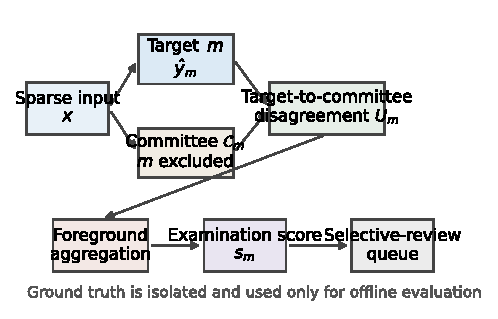
\includegraphics[width=0.98\columnwidth]{figure_framework_outlined.pdf}
 \caption{Target-specific scoring and offline evaluation. The target is excluded from its heterogeneous committee; ground truth is revealed only after scoring.}
 \label{fig:framework}
\end{figure}

\subsection{Target-specific disagreement family}
For generated voxel $i$, the default map is
\begin{equation}
 U_m(i)=\mathop{\mathrm{median}}_{b\in\mathcal C_m}
 |\hat y_m(i)-\hat y_b(i)|.
 \label{eq:score}
\end{equation}
This is a median target-to-committee difference, not statistical median absolute deviation and not posterior variance. Self-exclusion is essential because including $\hat y_m$ creates a structural zero. To separate the protocol from the elementary aggregator, define $d_{mb}(i)=|\hat y_m(i)-\hat y_b(i)|$ and
\begin{equation}
 U_m^g(i)=g\!\left(\{d_{mb}(i):b\in\mathcal C_m\}\right),
 \label{eq:family}
\end{equation}
where $g$ may be the median, mean, maximum, or trimmed mean. Comparators also include distance to the committee mean/median image, target-excluded committee spread, mean/median pairwise disagreement, residuals to linear/cubic interpolation, and gradient- or Laplacian-domain variants. These tests distinguish robust target conditioning from generic set dispersion, analytical departure, and local structural inconsistency. Changing the named target changes every $d_{mb}$ and may change the review order; a single all-output spread map cannot attribute risk to one interpolator.

\subsection{Generated support, masking, and intensity}
For factor $r$, let $\mathcal Z_{\rm obs}^{(r)}$ be the recorded anchor indices and $\mathcal Z_{\rm gen}^{(r)}=\mathcal Z\setminus\mathcal Z_{\rm obs}^{(r)}$. The audited runs begin at anchor $a=0$, hence $\mathcal Z_{\rm obs}^{(r)}=\{z:(z-a)\bmod r=0\}$; define $\mathcal G_r=\{i:i_z\in\mathcal Z_{\rm gen}^{(r)}\}$. Observed anchors are never scored. The default deployment mask and examination score are
\begin{align}
 M_m^{(r)}(i)&=\mathbf1\!\left[|\hat y_m(i)|>0.01\max_{j\in\mathcal G_r}|\hat y_m(j)|\right],\label{eq:mask}\\
 s_m^{(r)}&=\frac{\sum_{i\in\mathcal G_r}M_m^{(r)}(i)U_m(i)}{\sum_{i\in\mathcal G_r}M_m^{(r)}(i)}.
 \label{eq:case}
\end{align}
The formulation is independent of factor; $r$ only determines $\mathcal G_r$. Each factor forms a separate review queue because raw score scales need not be comparable. Foreground aggregation prevents background dominance, although a target mask may omit suppressed tissue. Ground-truth masks are rejected by the deployment path. Predictions share the source-volume intensity representation; independent output normalization is only a sensitivity because it can erase cross-model amplitude information.

\subsection{Identifiability and common-mode invariance}
Write $\hat y_b=y+c+\epsilon_b$, where $c$ is shared error and $\epsilon_b$ is member-specific. Then
\begin{equation}
 \hat y_m-\hat y_b=\epsilon_m-\epsilon_b.
 \label{eq:decomp}
\end{equation}
For any perturbation $c'$ applied identically to the target and every committee member on the evaluated support,
\begin{equation}
 U_m(\{\hat y_b+c'\})=U_m(\{\hat y_b\}),
 \label{eq:invariance}
\end{equation}
because each target-to-member difference is unchanged. This exact common-mode invariance is both the method's rationale and its blind spot: target-specific separation can be ranked, but shared deletion, blur, bias, or preprocessing failure is unidentifiable from disagreement alone. Committee diversity is therefore a necessary operating condition, not a guarantee that consensus is correct.

\subsection{Selective review and implementation separation}
Ground truth enters only offline. Let $E_j$ be foreground MAE for examination $j$. Sorting by increasing $s_m$ yields the retained set $A_q$ at coverage $q$ and risk
\begin{equation}
 R(q)=|A_q|^{-1}\sum_{j\in A_q}E_j.
\end{equation}
We report foreground pixel Pearson correlation, examination-level Spearman $\rho$, absolute retained MAE, $\mathrm{RRR}(q)=[R_{\rm random}-R(q)]/R_{\rm random}$, and
\begin{equation}
 \mathrm{nAURC}=\frac{\mathrm{AURC}-\mathrm{AURC}_{\rm oracle}}
 {\mathrm{AURC}_{\rm random}-\mathrm{AURC}_{\rm oracle}},
 \label{eq:naurc}
\end{equation}
where zero is oracle and one expected random review. Coverage is always the retained fraction; $1-q$ is referred. Only ordering is interpreted---the magnitude of $s_m$ is not an error probability. Computing Eq.~\eqref{eq:score} costs $O(|\mathcal G||\mathcal C_m|)$ and can stream members. The scoring API receives predictions and metadata only; ground truth, oracle ranking, and error-derived labels reside in a separate evaluator, preventing accidental leakage.

\section{Experiments}
\subsection{Cohorts, outputs, and frozen protocol}
The factor-four study uses IXI (115 examinations) \cite{ixi}, fastMRI-brain (24) \cite{zbontar2018fastmri}, and an internal NingXia cohort (22) pooled from eight held-out folds. IXI includes I$^3$Net, HAT, SwinIR, and ACSI; the other cohorts include the first three. Linear and cubic interpolation provide analytical references \cite{keys1981cubic,thevenaz2000interpolation,unser1999splines}, yielding 161 examinations and ten fixed profiles. The pre-declared cross-factor extension uses the identical fastMRI-brain and NingXia identities at $r\in\{2,4,6\}$ and freezes the common model set to I$^3$Net, HAT, SwinIR, linear, and cubic. A separate expanded sensitivity adds ArSSR, CycleINR, Pix2PixGAN, and SMamba-UNet only because all six aligned prediction sets exist; reconstruction fidelity was not used to select members.

\begin{table}[H]
 \centering
 \caption{Cohorts and stored neural outputs. Analytical references are available for every profile.}
 \resizebox{\columnwidth}{!}{\begin{tabular}{lcll}
\toprule
Cohort & $n$ & Neural target outputs & Evaluation design \\
\midrule
IXI & 115 & I$^3$Net, HAT, SwinIR, ACSI & fixed held-out outputs \\
fastMRI-brain & 24 & I$^3$Net, HAT, SwinIR & fixed stored outputs \\
NingXia & 22 & I$^3$Net, HAT, SwinIR & eight-fold out-of-fold \\
\bottomrule
\end{tabular}
}
 \label{tab:protocol}
\end{table}

All NIfTI identities, geometry, and generated indices are checked before scoring. The frozen configuration uses all non-target members, Eq.~\eqref{eq:score}, raw inverse-normalized intensity, the 1\% target mask, and 2,000 paired examination-bootstrap resamples. The cross-factor seed is 20260724; matched cases reuse bootstrap identities. Every legal factor-four committee subset is recomputed from voxel outputs. No external-test result changes the score, mask, or committee.

SwinIR flip-TTA is evaluated only where matching four-view maps exist. Pixel correlation is calculated per examination and aggregated by Fisher $z$; case ranking uses Spearman $\rho$ with paired bootstrap intervals. Identical bootstrap indices are reused for paired comparisons. Mask variants that alter the foreground support are summarized by score-rank stability and endpoint-specific intervals rather than invalid paired differences against a changed MAE definition. Highest-MAE-decile AUROC/AUPRC is secondary because the two smaller cohorts contain only three positives per target. No profile or examination is removed after observing its score, and no sensitivity result replaces the frozen primary configuration on an external cohort.

\subsection{Primary association and selective review}
\begin{table}[H]
 \centering
 \caption{All ten pre-specified profiles. Lower nAURC is better; coverage is retained fraction.}
 \resizebox{\columnwidth}{!}{\begin{tabular}{lcccc}
\toprule
Profile & Pixel $r_z$ & Case $\rho$ [95\% CI] & nAURC [95\% CI] & RRR$_{50}$ \\
\midrule
IXI/ACSI & 0.435 & 0.954 [0.925, 0.972] & 0.035 [0.018, 0.060] & 50.1\% \\
IXI/HAT & 0.512 & 0.966 [0.940, 0.980] & 0.024 [0.012, 0.042] & 49.6\% \\
IXI/I$^3$Net & 0.351 & 0.951 [0.922, 0.969] & 0.044 [0.024, 0.073] & 52.1\% \\
IXI/SwinIR & 0.520 & 0.965 [0.937, 0.980] & 0.025 [0.012, 0.044] & 49.5\% \\
\midrule
fastMRI/HAT & 0.328 & 0.916 [0.758, 0.962] & 0.067 [0.017, 0.176] & 19.7\% \\
fastMRI/I$^3$Net & 0.291 & 0.890 [0.713, 0.966] & 0.092 [0.029, 0.194] & 19.3\% \\
fastMRI/SwinIR & 0.363 & 0.931 [0.781, 0.978] & 0.061 [0.012, 0.150] & 20.5\% \\
\midrule
NingXia/HAT & 0.277 & 0.929 [0.790, 0.975] & 0.076 [0.016, 0.228] & 22.2\% \\
NingXia/I$^3$Net & 0.356 & 0.914 [0.769, 0.970] & 0.063 [0.016, 0.186] & 23.1\% \\
NingXia/SwinIR & 0.279 & 0.936 [0.807, 0.983] & 0.036 [0.007, 0.120] & 21.4\% \\
\bottomrule
\end{tabular}
}
 \label{tab:main}
\end{table}

Table~\ref{tab:main} shows moderate foreground localization (\PixelFisherRange) but strong examination ranking (\CaseSpearmanRange). Aggregation over generated foreground suppresses local noise and preserves between-case severity even when the map does not precisely identify each erroneous structure. nAURC is \NAURCRange; at 50\% retained coverage, referring the highest-score half lowers retained MAE by \RRRFiftyRange\ relative to random review. Confidence intervals are widest on fastMRI-brain and NingXia, so the continuous curves are more informative than a single threshold.

\begin{figure*}[!t]
 \centering
 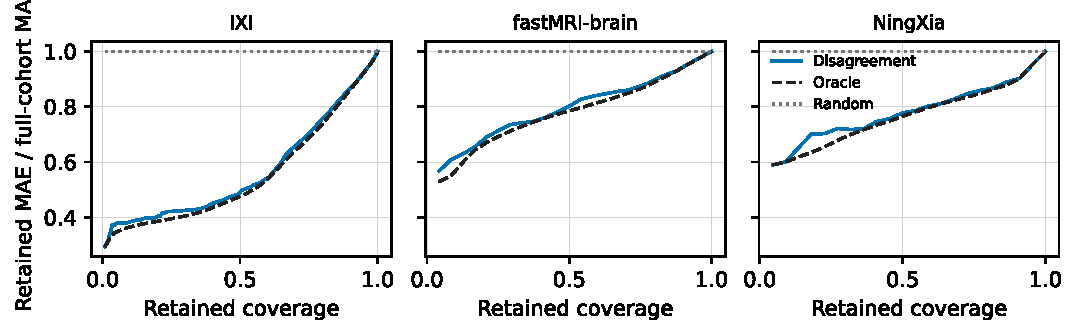
\includegraphics[width=0.82\textwidth]{figure_risk_coverage_outlined.pdf}
 \caption{Risk--coverage curves averaged over target interpolators after normalization by full-cohort MAE. The score remains between random and oracle review across cohorts; lower retained risk is better.}
 \label{fig:risk}
\end{figure*}

The complete curves in Fig.~\ref{fig:risk} avoid choosing a favorable test-set operating point. The largest absolute reduction occurs on IXI; smaller but consistent reductions occur on the two smaller cohorts. Because raw MAE is cohort-scale dependent, cross-cohort comparisons use nAURC and RRR rather than raw error.

\subsection{Score design, committee membership, and preprocessing}
\begin{table}[H]
 \centering
 \caption{Score and committee ablations averaged over fixed target profiles (nAURC; lower is better).}
 \resizebox{\columnwidth}{!}{\begin{tabular}{lll}
\toprule
Dataset & Score nAURC: med./mean/std. & Committee nAURC: neural/analytic/full \\
\midrule
fastMRI-brain & 0.073/0.070/0.074 & 0.017/0.118/0.073 \\
IXI & 0.032/0.043/0.049 & 0.033/0.059/0.032 \\
NingXia & 0.058/0.056/0.033 & 0.094/0.031/0.058 \\
\bottomrule
\end{tabular}
}
 \label{tab:ablation}
\end{table}

The median is a stable default but not a uniquely superior aggregator (Table~\ref{tab:ablation}). Across all 18 cross-factor profiles, its equal-profile $\Delta$nAURC versus mean is \MedianMeanDelta; versus target-invariant all-output spread it is \MedianSpreadDelta\ (negative favors median). Both intervals cross zero. The reliability signal is therefore not specific to the median, and target conditioning does not uniformly outperform generic examination difficulty. Committee composition is cohort dependent: neural peers are strongest on fastMRI-brain, analytical references on NingXia, and the full committee is near-best on IXI. Across legal factor-four subsets, nAURC spans 0.009--0.139; member identity matters more than size. The full committee is a frozen governance choice, not an empirical optimum.

Independent per-output normalization markedly degrades or reverses factor-four rankings, whereas input- and committee-derived masks largely preserve them. A common source-intensity representation is therefore part of the scoring contract; complete sensitivity results remain in the extended paper.

\subsection{Shared-error boundary and qualitative behavior}
The controlled stress test uses 20 fixed identity-sorted IXI examinations, all four targets, a foreground-constrained additive patch, five strengths, and a mask frozen before corruption. The target-specific arm perturbs only $\hat y_m$; the shared arm adds the identical patch to the target and every committee output.

\begin{figure}[H]
 \centering
 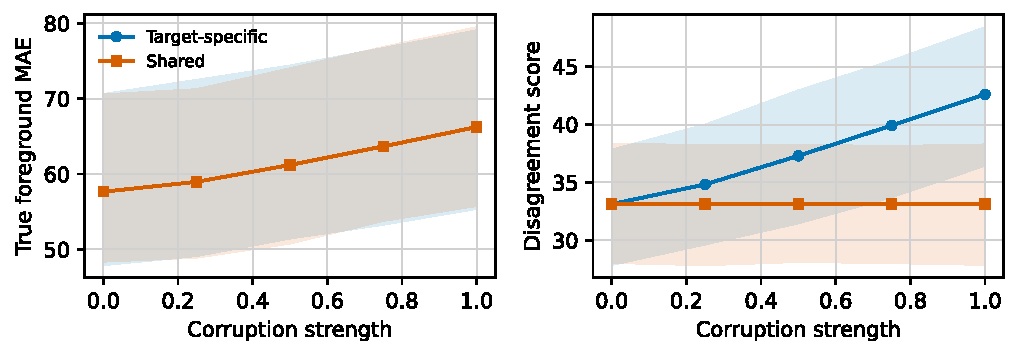
\includegraphics[width=0.98\columnwidth]{shared_error_stress_outlined.pdf}
 \caption{Controlled shared-error test. Target-specific corruption raises both MAE and disagreement; identical corruption of all outputs raises MAE while cancelling from target-to-member differences. Bands are 95\% bootstrap intervals.}
 \label{fig:stress}
\end{figure}

At maximum strength, target MAE rises by \StressMaeIncrease\ in both arms. Disagreement rises by \StressTargetIncrease\ for target-specific corruption but changes by \StressSharedChange\ under shared corruption, although mean committee MAE still rises by \StressCommitteeMaeIncrease. Figure~\ref{fig:stress} directly confirms Eq.~\eqref{eq:invariance}; it is an identifiability test rather than a simulation of all clinical failures.

\subsection{Cross-factor generalization and specificity}
\begin{figure*}[!t]
 \centering
 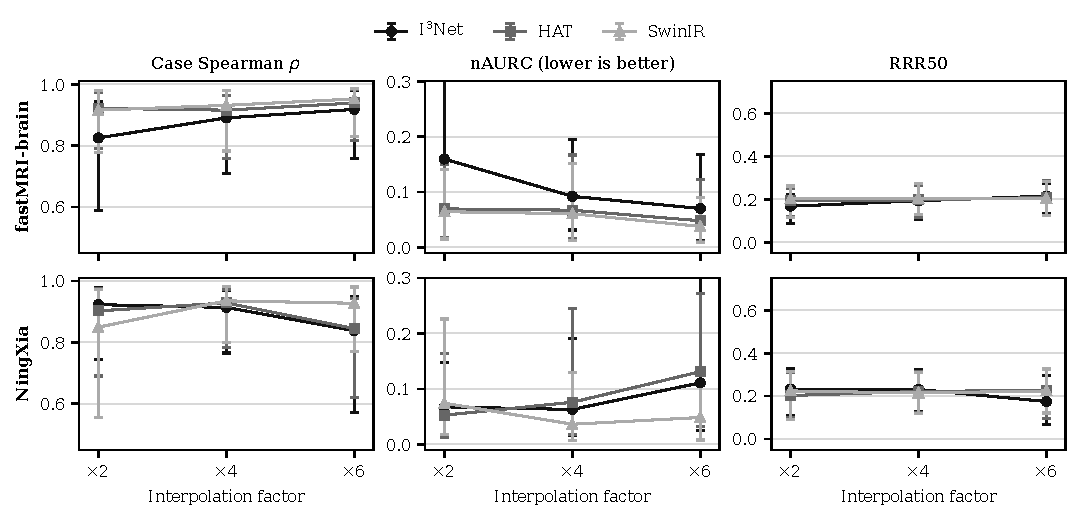
\includegraphics[width=0.94\textwidth]{cross_scale_figure.pdf}
 \caption{Frozen-committee reliability across factors. Points are target-specific estimates and bars are 95\% paired case-bootstrap intervals. Each factor forms its own review queue; lower nAURC is better.}
 \label{fig:crossscale}
\end{figure*}

Reconstruction MAE increases monotonically from $\times2$ to $\times6$ in both cohorts, but review ranking does not track difficulty monotonically (Fig.~\ref{fig:crossscale}). Target-averaged fastMRI-brain $\rho$/nAURC improves from 0.888/0.098 to 0.937/0.052. NingXia peaks at $\times4$ (0.926/0.058) and degrades at $\times6$ (0.871/0.097), while RRR50 remains 20.9\%; paired $\times6-\times4$ intervals do not establish degradation for every target. Thus $\times6$ retains useful ordering but reveals a cohort-dependent limit.

For direct target-specificity, we correlate each $s_m$ with every target model's true error. The matched-minus-mismatched advantage is only \MatchedAdvantageRange\ across six profiles, and every 95\% interval includes zero. The score ranks difficult examinations well but does not preferentially identify which of the three neural targets failed; shared case difficulty dominates. This negative result narrows the interpretation of ``target-to-committee'' from empirical attribution to an explicitly conditioned scoring construction.

\subsection{Single-model comparison and measured cost}
On the same 24 fastMRI-brain $\times4$ SwinIR examinations, four-view TTA yields $\rho=0.960$ and nAURC 0.023 versus 0.931 and 0.061 for committee scoring. The paired nAURC difference is $-0.038$ [95\% CI $-0.119$, 0.001], so the apparent gain is not conclusive. Stored-output auditing takes 1.18 s mean/2.87 s p95 per examination on CPU with 0.89 GiB peak RSS; online use additionally incurs every neural reconstruction.

\section{Discussion and Conclusion}
The evidence supports examination triage more strongly than precise voxel localization. A high $s_m$ prioritizes inspection while preserving the original reconstruction and committee identities; a low score indicates consensus only within the available committee. Coverage should follow review capacity rather than a retrospectively tuned error threshold, and a deployment threshold requires validation after changes in scanner, reconstruction software, intensity mapping, or committee membership.

The protocol is most attractive for retrospective audit, benchmark comparison, or systems that already cache several deterministic outputs. If only one model can be run, TTA, posterior sampling, acquisition residuals, or a validated error predictor may be more economical. A larger committee is not automatically better: member identity matters more than count, and the available no-reference diversity proxy cannot reliably choose the best compact subset. In practice, a review system should therefore freeze the committee specification, log member identities with every score, and monitor score distributions after software or acquisition changes rather than silently swapping members.

The score is also complementary to model-internal uncertainty. TTA probes sensitivity of one model to transformations, whereas cross-model disagreement probes separation from alternative reconstructions. Their failure modes need not coincide: one model may be unstable while peers agree, or all models may be confidently wrong together. A future deployment study should measure whether presenting both signals improves reviewer prioritization, review time, or downstream robustness without encouraging automation bias.

The principal limitations are structural. Shared errors are invisible, correlated members reduce diversity, a target mask can omit suppressed tissue, and unusual correct detail can be over-referred. Evidence remains restricted to T2 brain MRI; fastMRI-brain and NingXia are small, $\times6$ NingXia degrades, and the matched analysis cannot separate target identity from shared difficulty. There is no reader study or downstream task, and MAE is not diagnostic harm. Target-to-committee disagreement is therefore a reproducible ranking layer for selective review of stored outputs, not calibrated uncertainty, model attribution, or a clinical guarantee.

\clearpage
\bibliographystyle{IEEEbib}
\bibliography{references}
\end{document}
